\documentclass[sigconf]{acmart}

%%
%% \BibTeX command to typeset BibTeX logo in the docs
\AtBeginDocument{%
  \providecommand\BibTeX{{%
    \normalfont B\kern-0.5em{\scshape i\kern-0.25em b}\kern-0.8em\TeX}}}

\begin{document}

\title{Deep Learning on Edge Devices by Deep Compression}
\subtitle{a case study on medical image analysis on mobile phones}


\author{Wenjie Du}
\affiliation{%
  \institution{China University of Pretroleum}
}
\email{wenjay.du@gmail.com}

\author{Weishan Zhang}
\affiliation{%
  \institution{China University of Pretroleum}
}
\email{zhangws@upc.edu.cn}

\author{Yan Liu}
\affiliation{%
 \institution{Concordia University}}
 \email{yan.liu@concordia.ca}
 
 
\begin{abstract}
In recent years, deep neural networks have outperformed many traditional algorithms in many application scenarios like computer vision and natural language processing. Nowadays, not only in labs or in innovative projects, application of deep learning in the industries is also becoming increasingly widespread. However, there are also many limitations if you want to train and deploy them. Obtaining big datasets needed for successfully training DNNs is one of these limitations. Especially in some specified domains like medical industry, data from patients is heavily protected, that means training samples we can collect are limited. Another limitation is about hardware resources needed for running DNNs. It is a ground truth that DNNs are very demanding on computation and memory. As a result, deploying them on resource limited devices is a tough job, let alone edge devices such as mobile phones. In this paper, we first train a modified U-net \cite{improved-unet} on datasets of brain images and demonstrate it is more stable and robust than the original U-net\cite{unet}. We then study the combined use of filter reducing and channel pruning to further compress this improved U-net. Our experiments shows this combination can not only help decrease model sizes effectively, but also speed up inference of networks, while suffering little accuracy loss. Additionally, benchmark tests of inference time prove that this compression method makes it possible for our DNN models to run on edge devices and provide services.
\end{abstract}

\keywords{Deep Learning \and Model compression \and Medical Image}

\section{Introduction}
Recently, deep learning has achieved breakthrough development, especially in the field of computer vision, and now is helping people handle all kinds of tasks in all walks of life. Although deep networks outperform most traditional algorithms, there are some prerequisites that need to be met before application, and actually, some of them are quite troublesome. Firstly, it is widely accepted that thousands of annotated training samples are needed for successful training of DNNs. However, sample data collection is not something you can make as long as you want to, especially in the medical industry, where data from patients is protected well in consideration of privacy. Therefore, training of neural networks in the medical field often has insufficient datasets.

To handle this problem, data augmentation \cite{data-augmentation} is an effective method to help make the most of limited available datasets and increase the accuracy of neural networks. It is a ground truth that the more data a neural network can get access to during training, the better performance it can achieve. Based on data augmentation, a better way to solve this problem of insufficient training data is to design the correct neural network architecture according to the task to be processed. U-net[1] was proposed in 2015 and it was designed specifically for medical image processing, which can obtain good performance as trained with few training datasets. At that time, U-net outperformed the previous convolutional networks and ran faster than them as well.

As for the limit of the model size, lately, there has been rising interest in compressing models to accelerate them and to achieve smaller size. This is no surprise, because compression opens up more possibilities for practical applications, especially on mobile devices. Recent years witnessed significant progress in virtual reality, augmented reality, and smart wearable devices, creating unprecedented opportunities for researchers to tackle fundamental challenges in deploying deep learning systems to portable devices with limited resources (e.g. memory, CPU, energy, bandwidth)\cite{survey-of-compression}. And even a new class of efficient neural networks called MobileNets has been proposed to train models for embedded applications especially \cite{mobilenets}. Objectively speaking, incorporating models of DNNs into mobile APPs enables real time processing and data processing locally, which can bring better privacy protection and user experience. To obtain these benefits, model compression is necessary. For example, we all know that models generated by deep neural networks have big size, usually several hundreds MB, and they will take up considerable storage if you want to build APPs based on these big models. Let alone other restrictions such as in App Store, "apps above 100MB will not download until you connect to Wi-Fi"\cite{deep-compression}. Furthermore, storage is just one part of the problem. Generally, bigger size means needing more loading time and consuming more runtime resources such as memory, computational power and battery power. Compression can not only help reduce storage and energy, but also accelerate inference of models. Deep compression based on pruning, quantization and Huffman coding, proposed by Han et al., can significantly shorten the inference time of deep network models and can significantly decrease the size of models likewise, without impacting accuracy\cite{deep-compression}.

Recent CNN acceleration works fall into three categories: optimized implementation, quantization, and structured simplification that convert a CNN into compact one \cite{channel-pruning}. To simplify the structure, decreasing the number of filters in each layer is a straightforward and simple method, which can reduce the number of parameters in the network directly. But less parameters doesn't necessarily mean poor performance. Although there is a widely accepted opinion that is the network having more parameters can learn more complex functions. There is someone having proved that shallower or smaller neural networks with much fewer parameters trained in appropriate ways can also achieve no less performance than deeper and bigger ones with much higher capacity, such as Lei Jimmy Ba and Rich Caruana\cite{really-need-to-be-deep}, and Hao Zhou et al.\cite{less-is-more}.

In this paper, we study the feasibility of compressing U-net and running it on mobile devices. We first show that the improved U-net architecture presented by Karttikeya Mangalam et al.\cite{improved-unet} has more stability and robustness than the original U-net . Then we reduce the starting filter quantity according to the characteristic of the U-net structure to prove that even with much less filters of each layer in U-net, which also means less parameters and simpler architecture, it can still achieve good performance. At last, we combine the filter reducing and channel pruning to further compress our U-net model to enable it to run better on embedded devices.

\section{Methodology}
\subsection{U-net}
Built upon full convolutional network\cite{fcl4seg}, U-net proposed by Olaf Ronneberger et al.\cite{unet} , consists of a contracting path and an expanding path. U-net starts with the first layer whose channel depth is 64, and doubles the depth in 4 following layers in the contracting path to capture context from inputs, until reaching 1024 at the bottom. And then the number of filters is reduced back to 64 in the expanding path, which enables precise localization. Therefore, the whole architecture is U-shaped, as is shown in Fig. \ref{fig:fig1}(left) below. 

The most obvious features of U-net are its U-shaped architecture and skip connections. The contracting path can be seen as an encoder, which down-smaples inputs 4 times and help us extract advanced semantics from inputs. The expanding path on the right works as a decoder, which up-samples inputs 4 times to increase the resolution of outputs. As for the skip connections, they can transfer information from layers of the contracting path to those of the expanding path that are on the same stage with the former. Just like in ResNet\cite{resnet}, these skip connections guarantee more information can reach higher layers and combine with up-sampled output. These 2 main features ensure the good performance of U-net.


\begin{figure}
  \centering
  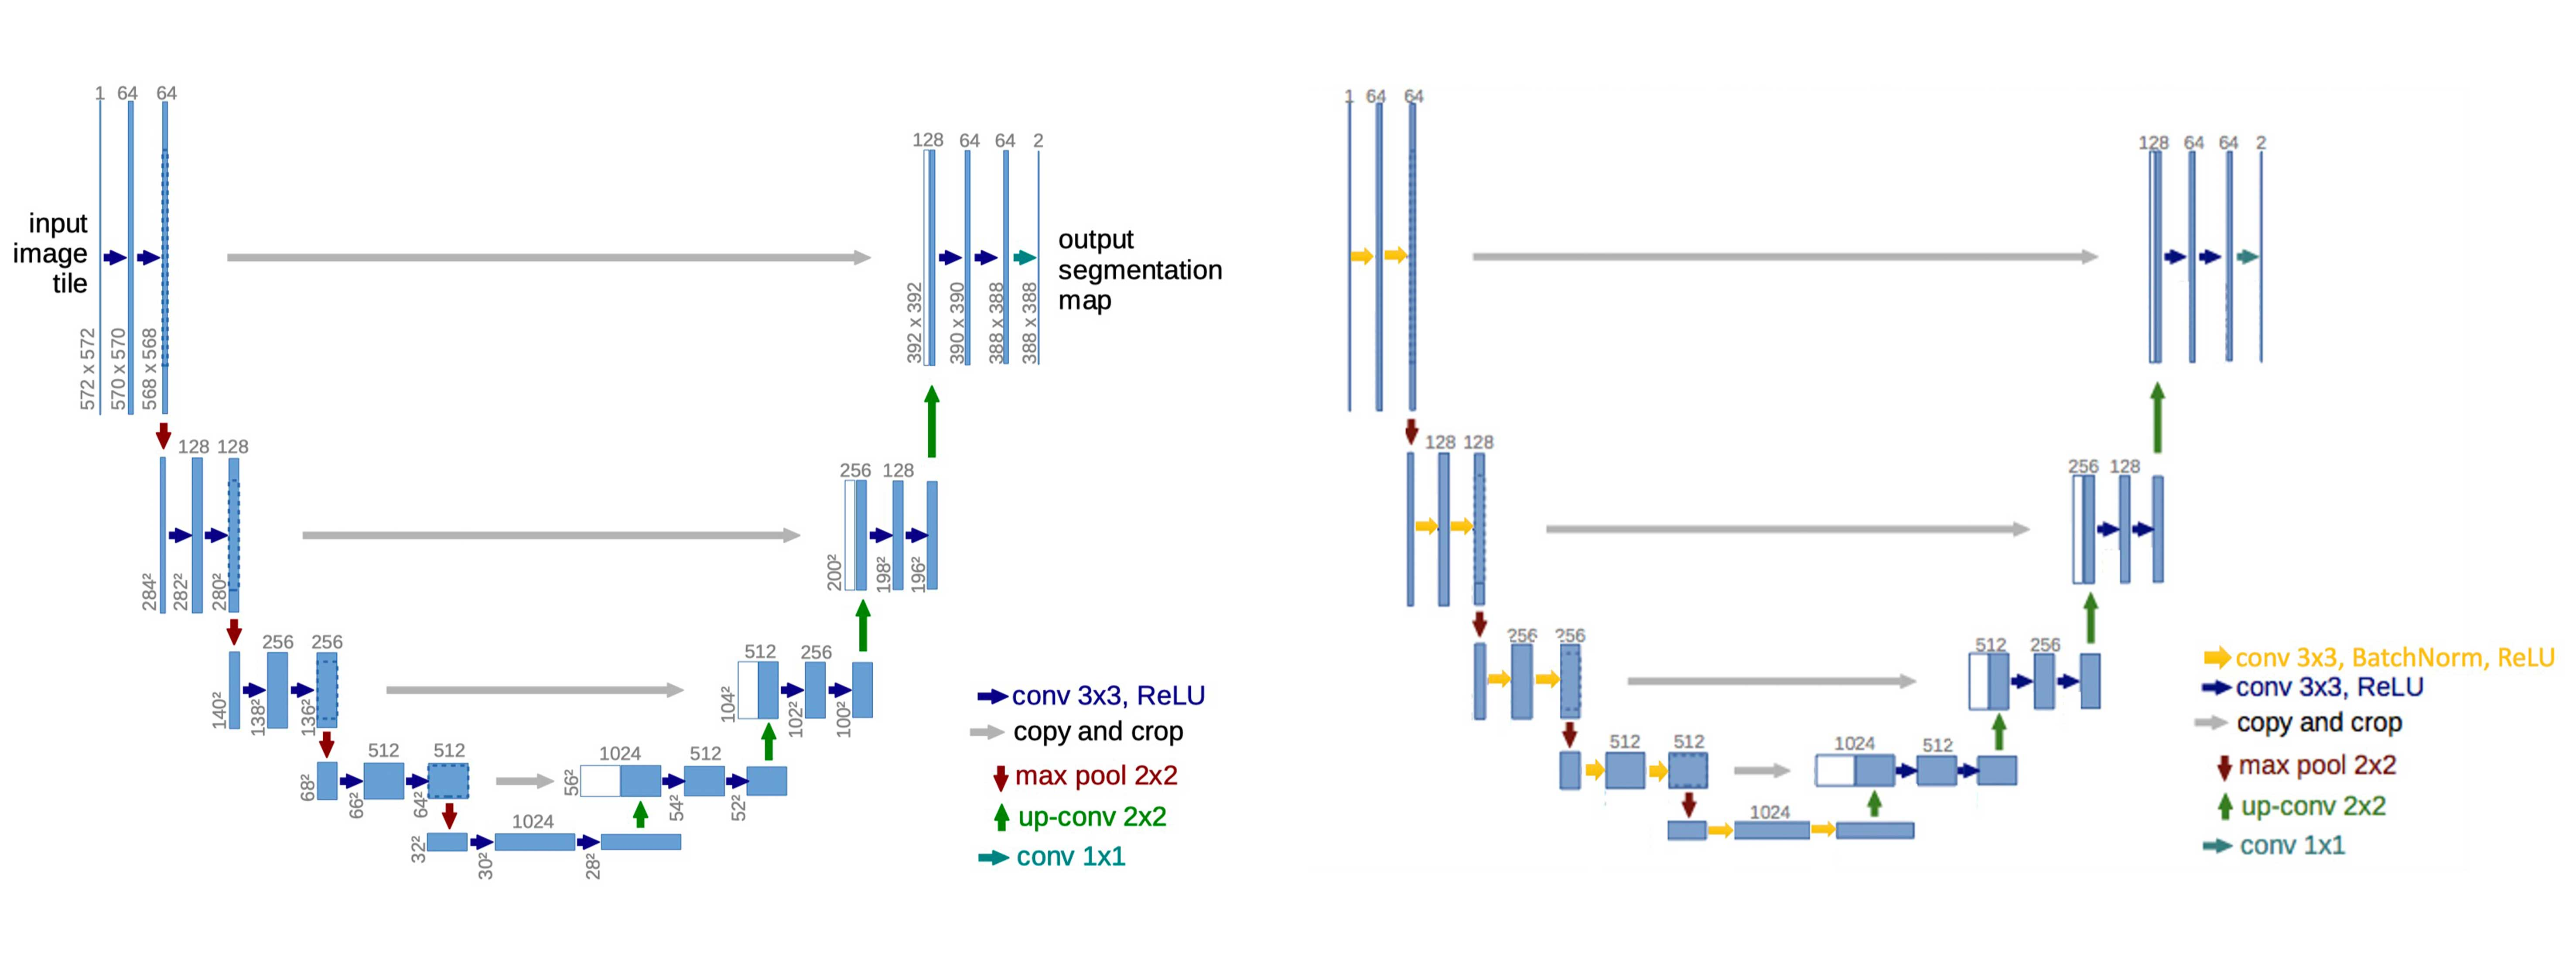
\includegraphics[width=15cm]{fig1.jpg}
    \caption{ Left: the original U-net architecture; Right: the improved U-net architecture with batch normalization added to corresponding locations in the contracting part.}
  \label{fig:fig1}
\end{figure}

\subsection{Improved U-net}
Here, we adopt an improved U-net architecture presented by Karttikeya Mangalam et al.\cite{improved-unet}. They added batch normalization to the corresponding locations in the contracting path of the original U-net architecture, just as shown in Fig. \ref{fig:fig1}(right). Those golden arrows are modifications where they added batch normalization. 

Batch normalization was initially introduced by Sergey Ioffe and Christian Szegedy\cite{batch-normalization} in 2015 to reduce the internal covariate shift, which is referred to the phenomenon of changes in distributions of each layer's inputs during training, caused by changes happening in nodes of previous layers. Internal covariate shift makes it difficult to train models, mainly because it forces us to train with lower training rate and to tune our networks carefully. Adding batch normalization before layers can help normalize the input. Hence, it is capable of alleviating the internal covariate shift, and speedup and simplify the training process. 

It is noteworthy that different from the original U-net architecture which has a dropout layer at the end of the contracting path, we still use batch normalization there. Dropout was brought by Srivastava et al. in 2014 \cite{dropout} as a simple way to prevent neural networks from over-fitting. It is capable of preventing complex co-adaptations to help reduce over-fitting. Co-adaptation is referred as connections between neurons make them be influenced by each other and neurons' behavior becomes highly correlated in the training context, while the performance will drop dramatically in the test context. What dropout does is randomly drop neurons with their connections while training, and this breaks up co-adaptations effectively, thus achieves the goal of alleviating over-fitting.

However, after batch normalization proposed, dropout becomes gradually replaced by it, not only because batch normalization achieves some same goals as dropout, but also because when they are combined, the combination often results in a worse performance rather than better together like what we think. Investigated by Xiang Li et al.\cite{disharmony}. This unexpected phenomenon is caused by differences between their test policies, which will lead to improper variance shift while the network is making inference. As a result, we adopt batch normalization in the architecture of improved U-net uniformly.

\subsection{Filter Reducing}
Based on the original U-net architecture, we reduce the number of filters in each layer. For example, the original U-net architecture starts with a channel depth of 64 in the first layer, i.e. the number of filters in the first layer is 64. More filters, more parameters, bigger models. Therefore, we reduce the number of filters and start with the first layer with a shallower depth. In the meanwhile, the strategy of increasing filter quantity is the same with the original architecture, doubles the number of filters in following each layer of the contracting path and reduces back in the expanding path. 

Actually, although this modification is common and simple, it works pretty well. Specific data is shown in Table \ref{tab:table1},\ref{tab:table2} and Fig. \ref{fig:fig2},\ref{fig:fig3}.

\subsection{Channel Pruning}

Pruning was firstly introduced by LeCun et al. in 1989 as a method called Optimal Brain Damage\cite{optimal-brain-damage} to eliminate connections in the network based on the Hessian of the loss function. This can accomplish the goal of shrinking size of models and handle the problem of over-fitting. Now it has been adopted widely in the research of model compression. Several variants like \cite{channel-pruning}\cite{pruning-filters}\cite{dis-channle-pruning} have been proposed to get better performance or achieve specified goals, like to be compatible with various network architectures. However, the core idea of them are consistent, that is to remove weights, whose value is lower than a given threshold and thus considered redundant and non-informative of the network. This operation is capable of simplifying the internal structure of neural networks, at the meantime, can reduce the computational complexity as well.

Inspired by improvements obtained by feature map reconstruction\cite{accelerating-deep-cnn}, which is used to reduce the accumulated error in the multi-layer neural network, He et al. introduced a channel pruning method in 2017 \cite{channel-pruning} to efficiently prune a trained convolution neural network at inference time. This method has 2 steps, channel selection and feature map reconstruction. The first step is to address the problem of which channels are proper and ought to be kept to maintain the network performance, and which channels are redundancy and should be removed to simplify the internal architecture. One challenge of channel pruning is removing channels in one layer may dramatically change the output, which is the input of the following layer and the output of the following layer will also have great changes. This ripple effect will affect the entire network. To avoid it, He et al. designed a method based on LASSO regression to find out those most representative channels and keep them. Those identified as redundant will be pruned, together with those channels taking them as input and filters producing them. The other step is to reconstruct the feature map with remaining channels. Actually, the first stop serves the second one. Experiments indicates that channel selection in the first step is necessary, because it imposes a big influence on the reconstruction error.

\subsubsection{Formulation}
Since the method has two steps, the algorithm also has two parts. Firstly, to figure out which channels are most representative, we have to obtain feature map of each channel, and then make judgments based on them. Here, we denote the input of each convolutional layer as $\mathcal{X} \in \mathbb{R}^{N \times h_{i} \times w_{i} \times c_{i}}$, where $N$ is the number of samples, $h_{i}$ and $w_{i}$ are the spatial size (height and width), and $c_{i}$ is the number of channels. And the convolutional filters is write as $\mathcal{W} \in \mathbb{R}^{k_{h} \times k_{w} \times c_{i} \times c_{o}}$, and similiarly $k_{i}$ and $k_{i}$ are the kernel size, and $c_{0}$ is the number of output channels.

Applying $X\times W$, ie. imposing convolutional operation on them, will produce $N\times n$ output martrix $Y$, which can be denoted as ${Y} ={X} \times {W} = \mathbb{R}^{N \times h_{o} \times w_{o} \times c_{o}}$. Here, ${X}$ can be sliced into ${X_i}$, the $i$-th channel of ${X}$, ${i}$=1,...,${c_i}$. Accordingly, ${W}$ can be dividec into ${W_i}$, the $i$-th channel of ${W}$, ${i}$=1,...,${c_i}$. Then the calculation formula of feature map outputted from the $i$-th channel can be written as 

\begin{equation}
\mathbf{Y} = \sum\nolimits_{i = 1}^{c_{i}} \mathbf{X}{i} \mathbf{W}{i}
\end{equation}

To remove redundant channels and minimize construction error simultaneously, the whole problem can be denoted as following: 

\begin{equation}
\underset{\boldsymbol{\beta}, \mathrm{W}}{\arg \min } \frac{1}{2 N}\left\|\mathrm{Y}-\sum_{i=1}^{c} \beta_{i} \mathrm{X}_{\mathrm{i}} \mathrm{W}_{\mathrm{i}}^{\top}\right\|_{F}^{2}+\lambda\|\boldsymbol{\beta}\|_{1}, \text { subject to }\|\boldsymbol{\beta}\|_{0} \leq c_i^{\prime}
\end{equation}

where ${\beta_i}$ is a binary-valued mask vector of ${c_i}$ dimension introduced to indicate whether the ${c_i}$ channel could be safely pruned (${\beta_i}$=0) or not (${\beta_i}$=1) from feature map. And ${\lambda}$ is penalty coefficient of ${l_1}$ regularization, which is used to control the num of zero terms in ${\beta}$ - larger ${\lambda}$, more zero terms in ${\beta}$ and higher speed-up ratio. This problem can be handled with two steps as follows.

Firstly, fix $W$ and solve $\beta$ to select channels. This can be tackled by applying LASSO regression.

\begin{equation}
\hat{\boldsymbol{\beta}}^{L A S S O}(\lambda)=\underset{\boldsymbol{\beta}}{\arg \min } \frac{1}{2 N}\left\|\mathrm{Y}-\sum_{i=1}^{c} \beta_{i} \mathrm{X}_{\mathrm{i}} \mathrm{W}_{\mathrm{i}}^{\top}\right\|_{F}^{2}+\lambda\|\boldsymbol{\beta}\|_{1}, \text { subject to }\|\boldsymbol{\beta}\|_{0} \leq c_i^{\prime}
\label{equ: equation1}
\end{equation}

Secondly, after channels are selected in the previous step, $\beta$ is now fixed and $W$ can be solved, or in other words, its value will be reassigned. The optimized solution can be found by least squares: 
\begin{equation}
\underset{\mathbf{W}^{\prime}}{\arg \min }\left\|\mathbf{Y}-\mathbf{X}^{\prime}\left(\mathbf{W}^{\prime}\right)^{\top}\right\|_{F}^{2}    
\end{equation}



\section{Experiments}
\subsection{Datasets}
In our experiments, we trained U-nets on two datasets. One is as referred to before, a dataset containing magnetic resonance brain images from HCP (Human Connectome Project)\cite{hcp}. Another is SORTEO (Simulation Of Realistic Tridimensional Emitting Objects) dataset\cite{sorteo}. Both of them are magnetic resonance brain image datasets and are organized according to BIDS (the Brain Imaging Data Structure), which is a standard format for organizing and describing datasets of neuroimaging experiments, developed under the circumstance that although MRI(Magnetic Resonance Imaging) is usually used to obtain the data for neuroimaging researches, no widely adopted standard for organizing collected data hinders researchers from sharing and reusing data\cite{bids}. Frankly, this standard structure make it easier to prepare data for training usage

In terms of sample quantities, the number of training samples, validation samples and test samples is 12470, 2418, 1744 respectively in HCP dataset. In SORTEO dataset, the number is 2034, 678, 678 respectively.

\subsection{Reduce the starting quantity of filters}
We implement both the original U-net and the improved U-net with Keras, and then reduce the quantity of filters of the first layer, then get 14 networks in total. We train them separately on both HCP and SORTEO datasets and achieve models in hdf5 format generated by Keras directly.

Taking a look at U-nets trained on the HCP dataset, as is shown in Table \ref{tab:table1}, firstly, it is obvious that improved U-net performs better than the original one, which suggests that the improved structure does work, especially when the number of filters is very small, for instance, while the starting quantity of filters is only one, the accuracy of the improved U-net still remains above 90 percent, but the accuracy original U-net can only obtain is 87.4 percent. Secondly, the model size in Table \ref{tab:table2} shrinks significantly as the number of filters decreases. Taking the improved U-net with 2 filters in the first layer as an example, its accuracy is 97.7\%, only 1.5\% lower than the improved one starting with 64 filters, but its size is 717.46 times smaller than the latter one. This seems very cost-effective, because all you need to do is to reduce the number of filters.

\begin{figure}
  \centering
  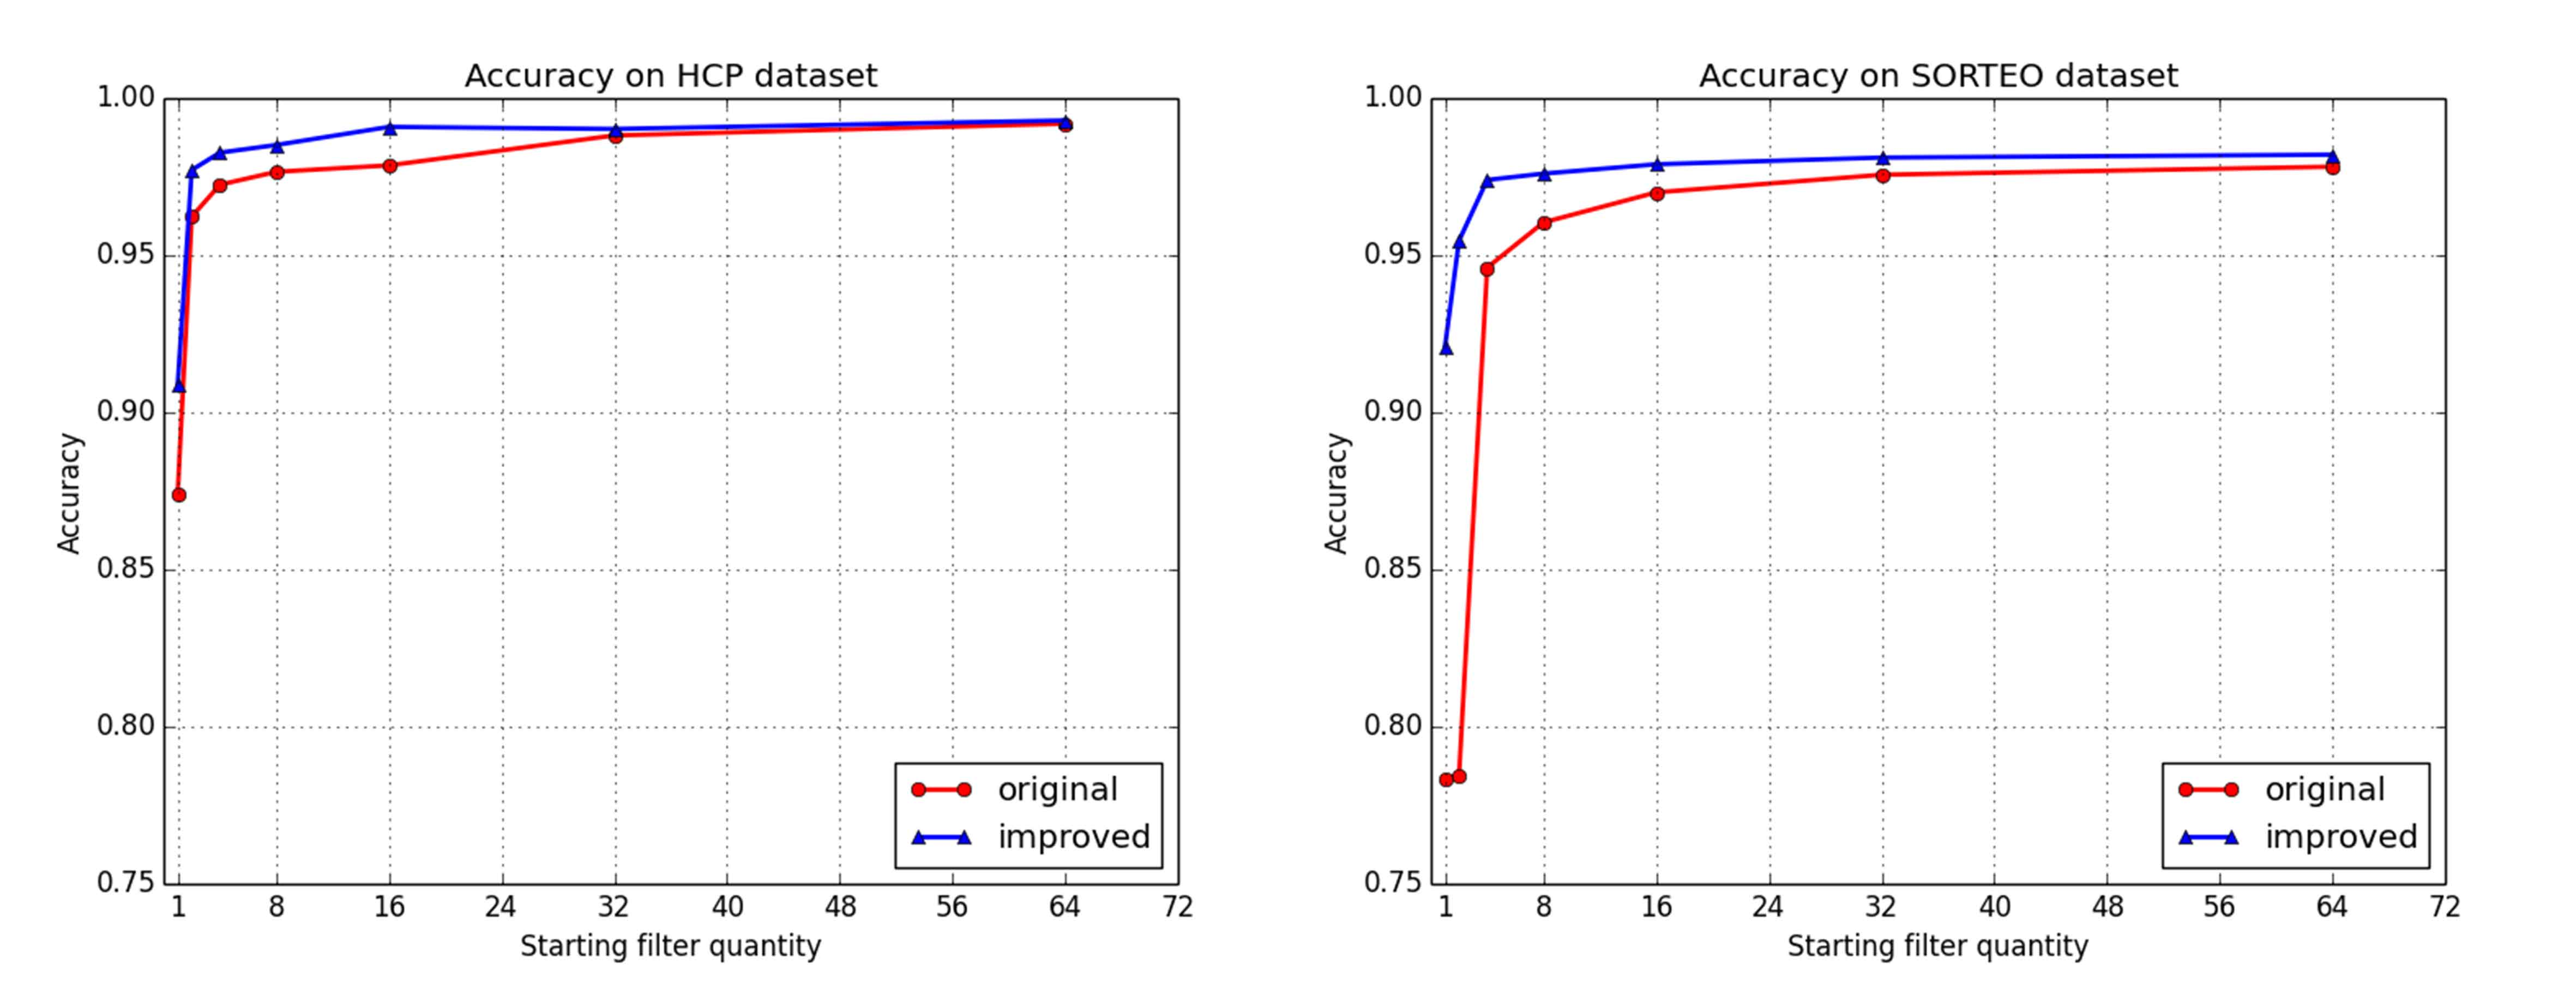
\includegraphics[width=15cm]{fig2.jpg}
    \caption{The left shows accuracy of both original U-net and improved U-net trained on HCP dataset as the starting filter quantity increases. The right shows the same content, just trained on the SORTEO dataset.}
  \label{fig:fig2}
\end{figure}

\begin{figure}
  \centering
  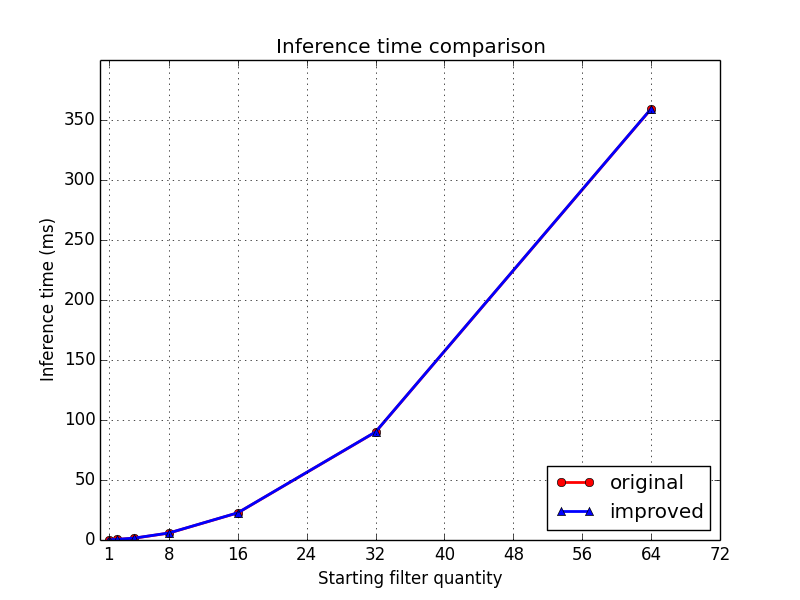
\includegraphics[width=9cm]{fig3.png}
    \caption{Model size increases significantly as the quantity of starting filters rises up. Moreover, in spite of the obviously better performance brought by the improved U-net, the increased models size is so small that can be neglectable. As shown in the above diagram, two lines almost overlap.}
  \label{fig:fig3}
\end{figure}

\begin{table}
 \caption{Performance of both U-net On HCP dataset}
  \centering
  \begin{tabular}{llll}
    \toprule
    Architecture & Starting quantity of filters & Test loss / Test accuracy  & Size of model in hdf5 format (MiB) \\
    \midrule
    original & 64 & 0.02062 / 0.99188 & 359.23     \\
    \midrule
    improved & 64 & 0.01782 / 0.99292 & 359.38     \\
    \midrule
    original & 32 & 0.02963 / 0.98815 & 89.93  \\
    \midrule
    improved & 32 & 0.02556 / 0.99020 & 90.04  \\
    \midrule
    original & 16 & 0.05149 / 0.97862 & 22.60  \\
    \midrule
    improved & 16 & 0.02388 / 0.99087 & 22.68  \\
    \midrule
    original &  8 & 0.06007 / 0.97657 & 5.76  \\
    \midrule
    improved &  8 & 0.03917 / 0.98511 & 5.83  \\
    \midrule
    original &  4 & 0.06907 / 0.97246 & 1.54  \\
    \midrule
    improved &  4 & 0.04389 / 0.98268 & 1.61  \\A
    \midrule
    original &  2 & 0.12175 / 0.96232 & 0.50  \\
    \midrule
    improved &  2 & 0.06026 / 0.97716 & 0.50  \\
    \midrule
    original &  1 & 0.19351 / 0.87413 & 0.23  \\
    \midrule
    improved &  1 & 0.17003 / 0.90861 & 0.23  \\
    \bottomrule
  \end{tabular}
  \label{tab:table1}
\end{table}


\begin{table}
 \caption{Performance of both U-net On SORTEO dataset}
  \centering
  \begin{tabular}{llll}
    \toprule
    Architecture & Starting quantity of filters & Test loss / Test accuracy  & Size of model in hdf5 format (MiB) \\
    \midrule
    original & 64 & 0.05706 / 0.97820 & 359.23 \\
    \midrule
    improved & 64 & 0.04674 / 0.98202 & 359.38 \\
    \midrule
    original & 32 & 0.06521 / 0.97563 & 89.93 \\
    \midrule
    improved & 32 & 0.04937 / 0.98110 & 90.04 \\
    \midrule
    original & 16 & 0.07996 / 0.97003 & 22.60 \\
    \midrule
    improved & 16 & 0.05525 / 0.97897 & 22.68 \\
    \midrule
    original &  8 & 0.09805 / 0.96047 & 5.76 \\
    \midrule
    improved &  8 & 0.06379 / 0.97600 & 5.83 \\
    \midrule
    original &  4 & 0.12937 / 0.94609 & 1.54 \\
    \midrule
    improved &  4 & 0.06849 / 0.97399 & 1.61\\
    \midrule
    original &  2 & 0.30759 / 0.78452 & 0.50 \\
    \midrule
    improved &  2 & 0.18313 / 0.95466 & 0.50\\
    \midrule
    original &  1 & 0.65986 / 0.78322 & 0.23 \\
    \midrule
    improved &  1 & 0.22036 / 0.92084 & 0.23\\
    \bottomrule
  \end{tabular}
  \label{tab:table2}
\end{table}

Above experimental data not only indicates that utilizing the method of reducing the filter number in the first layer can make networks extremely smaller with little loss in accuracy, but also reveals stability and robustness of the improved U-net in contrast with the original structure, because as is shown in Fig. \ref{fig:fig4}, it is clear that even trained on the much smaller SORTEO dataset and having only 1 filter in the 1st layer, the improved U-net can still achieve over 92\% accuracy, as the original one gets only 78 percent. 

\subsection{Continue to compress with channel pruning}
With the instruction of data from previous experiments, we know that the improved U-net is a better choice than the original. Now that we want to get as high accuracy as possible and as small model size as possible at the same time, we adopt the improved U-net architecture in this section of experiments. 

Here we use PocketFlow framework\cite{pocketflow} to implement channel pruning. PocketFlow is an open-source automated framework developed by Tencent to compress and accelerate neural networks. With the well implemented channel pruning algorithm[\ref{equ: equation1}] in PocketFlow, we can experiment with less more effort.

Firstly, we train the full precision models implemented with TensorFlow. Experimental data in Table \ref{tab:table3} shows that accuracy drops little as the starting quantity of filters decreases from 64 to only 1. Secondly, we prune half of channels channels of all models and results are recorded in Table \ref{tab:table4}. As data in both tables directly shown in Fig. \ref{fig:fig4}, we can easily find that channel pruning can significantly reduce mode size while the size of model is big, which means there is a large num of redundant parameters. Therefore, pruning can remove them effectively. But as the model size decreases, the quantity of redundant parameters also drops. As a result, influence of channel pruning is weakened. As for accuracy, loss caused by channel pruning is little, except the model with 1 filter in the first layer. Loss of accuracy in this model is huge, about 18.5\%. We hypothesize that the quantity of parameters in this network is originally small. After pruning, many parameters are removed and the left are not enough to maintain the high performance. Hence, its accuracy drops dramatically. It is not the model we actually want.


\begin{table}
 \caption{Performance of full-precision improved U-net On SORTEO dataset}
  \centering
  \begin{tabular}{llll}
    \toprule
    Architecture & Starting quantity of filters & Test accuracy  & Size of model in pb format (MiB) \\
    \midrule
    improved & 64 & 0.97641 & 164.19 \\
    \midrule
    improved & 32 & 0.97567 & 59.43 \\
    \midrule
    improved & 16 & 0.97579 & 33.23 \\
    \midrule
    improved &  8 & 0.97562 & 26.68 \\
    \midrule
    improved &  4 & 0.97305 & 25.04\\
    \midrule
    improved &  2 & 0.97143 & 24.63\\
    \midrule
    improved &  1 & 0.96695 & 24.52\\
    \bottomrule
  \end{tabular}
  \label{tab:table3}
\end{table}


\begin{table}
 \caption{Performance of channel-pruned improved U-net On SORTEO dataset}
  \centering
  \begin{tabular}{llll}
    \toprule
    Architecture & Starting quantity of filters & Test accuracy  & Size of model in pb format (MiB) \\
    \midrule
    improved & 64 & 0.97676 & 94.38 \\
    \midrule
    improved & 32 & 0.97536 & 41.98 \\
    \midrule
    improved & 16 & 0.97445 & 28.87 \\
    \midrule
    improved &  8 & 0.97406 & 25.59 \\
    \midrule
    improved &  4 & 0.96842 & 24.77\\
    \midrule
    improved &  2 & 0.96728 & 24.56\\
    \midrule
    improved &  1 & 0.78149 & 24.51\\
    \bottomrule
  \end{tabular}
  \label{tab:table4}
\end{table}

\begin{figure}
  \centering
  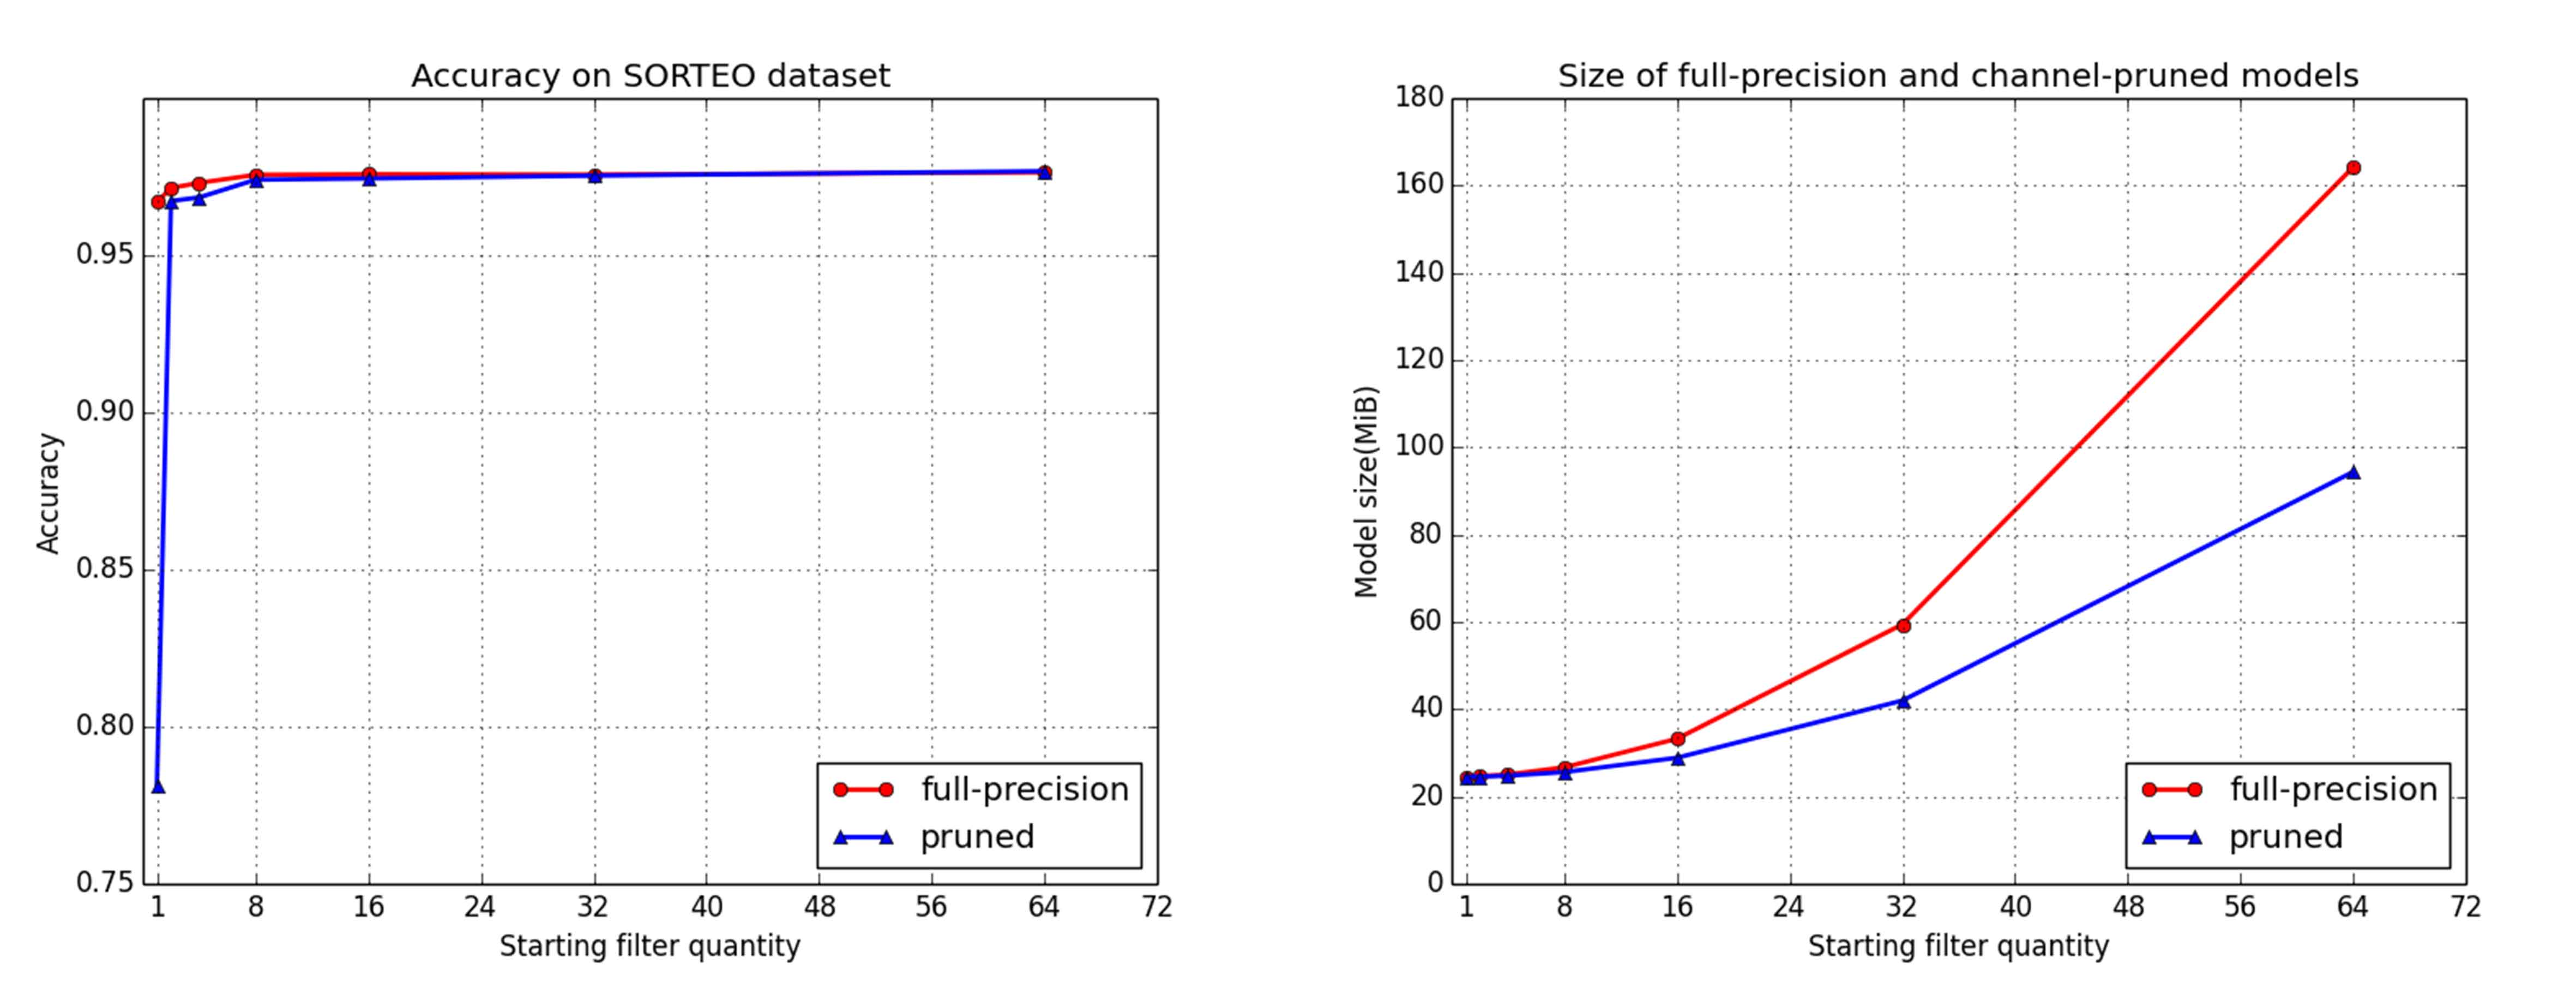
\includegraphics[width=15cm]{fig4.jpg}
    \caption{The left shows changes in accuracy of full-precison models and channel-pruned models trained on SORTEO dataset with the starting filter quantity increasing. The right shows changes in sizes of models.}
  \label{fig:fig4}
\end{figure}


\subsection{Benchmark tests of inference time on Raspberry Pi}
Raspberry Pi is a series of small single-board computers. The original purpose of developing it is to lower the cost of the education of computer science and promote it. Raspberry Pi is as fully functional as a full-size desktop computer, thought it is quite small, approximately credit-card sized. Nowadays, Raspberry Pi is so popular that it has become the representative of single-board computers and is widespreadly used in building robotics and intelligent cars. 

The one on our hand is a Raspberry Pi 3 Model B, which has a Quad-Core 1.2GHz Broadcom BCM2837 64bit CPU and 1GB RAM. Actually, available hardware resources on this micro computer are much few than on today's smartphones, especially in terms of RAM. 

In our experiments, we export our models into tflite format to enable them to run on our embedded device and then make benchmark tests of inference time on these models. Data shows that pruned models can run much more faster than full-precision models. Excluding the model with 1 starting filter that has been eliminated, results of test are shown in Table \ref{tab:table5} and Fig. \ref{fig:fig5} clearly reveals changes in inference time. The pruned model staring the 8 filters, which we  is approximately 35 times faster than the biggest full-precision model, but with neglectable loss in accuracy. All these result demonstrates that our work successfully achieves our goal that compress the size of the trained model and accelerate their speed with little accuracy loss.

\begin{table}
 \caption{Benchmark tests of inference time on Raspberry Pi}
  \centering
  \begin{tabular}{llll}
    \toprule
    Architecture & Starting quantity of filters & Inference time (ms)  & Size of model in tflite format (MiB) \\
    \midrule
    improved, pruned & 64 & 3653.20 & 69.89 \\
    \midrule
    improved, pruned & 32 & 805.94 & 17.50 \\
    \midrule
    improved, pruned & 16 & 346.35 & 4.40 \\
    \midrule
    improved, pruned &  8 & 150.36 & 1.12 \\
    \midrule
    improved, pruned &  4 & 108.18 & 0.30 \\
    \midrule
    improved, pruned &  2 & 82.81 & 0.09 \\
    \midrule
    improved, full\_precision & 64 & 5276.35 & 137.04 \\
    \midrule
    improved, full\_precision & 32 & 2850.60 & 34.29 \\
    \midrule
    improved, full\_precision & 16 & 1142.69 & 8.60 \\
    \midrule
    improved, full\_precision &  8 & 432.22 & 2.17 \\
    \midrule
    improved, full\_precision &  4 & 195.12 & 0.56 \\
    \midrule
    improved, full\_precision &  2 & 141.35 & 0.16 \\
    \bottomrule
  \end{tabular}
  \label{tab:table5}
\end{table}

\begin{figure}
  \centering
  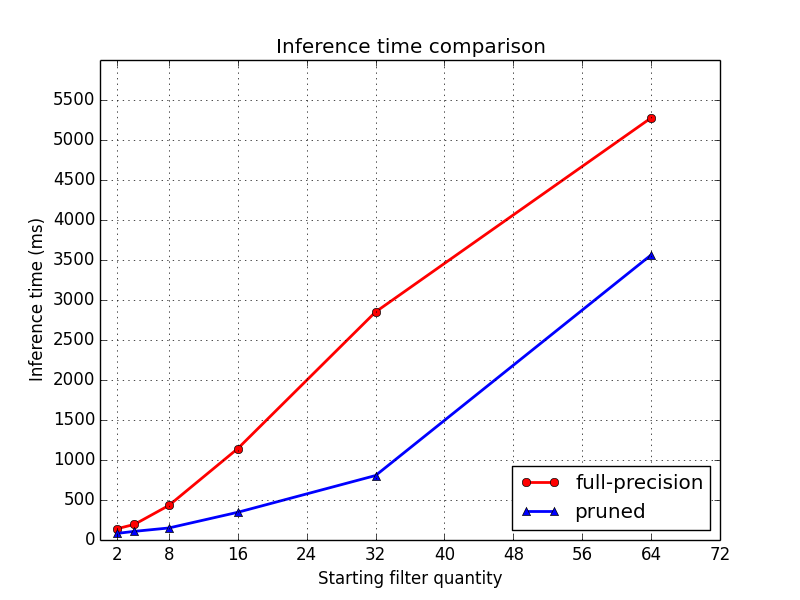
\includegraphics[width=15cm]{fig5.png}
    \caption{The left shows benchmark tests of inference time on Raspberry Pi. The right shows sizes of tflite models.}
  \label{fig:fig5}
\end{figure}

\section{Future work}
The above content has demonstrated that it is feasible to enable models of deep neural networks to run on embedded devices and they works quite well, though resources on these devices are restricted. Recently, developers in different fields are trying to combine machine learning with traditional industries. Until now, applications of those combinations are changing our life, making life more intelligent and brining us more convenience. 

Our idea is to develop an intelligent multi-function medical image processing system that combining machine learning with medical image processing and then stuff it into our mobile phones as an APP. Here, our model trained on magnetic resonance brain images is able to segment different parts of brains. Although the function of this model is simple and single, we can train different models able to process different kinds of medical images respectively and then compress them to lower the cost of entry to running these models. Finally, integrate them together as an ensemble of models, and this is the core part of this system.

This intelligent medical image processing system can enable people to make diagnoses without the help from doctors. Imagine that anyone, no matter he is a doctor or not, takes a photo of the medical image such as x-ray of a leg or MRI of the brain with he mobile phone, and open this photo in our APP, then the APP will give a result to him like whether the leg is fractured and where is fractured or whether there is a tumor in the brain. From doctors' point of view, with the highlighted affected part made by the system, doctors can explain their diagnosis to patients more clearly as well. In addition, this system can also be applied to medical education. With it, not only students can be guided to diagnose various conditions based on medical images, but also teachers can make more clear explanations to students with outputs from our system. 

\section{Conclusion}
In this paper, we trained an improved U-net\cite{improved-unet} on magnetic resonance brain image datasets and then imposed a combination of filter reducing and channel pruning to compress models to enable them to run on devices with limited hardware resources. Our experiments demonstrate that it is feasible to highly compress the U-net and deploy the model on embedded system with very restricted resources. In the future, we hope to further improve our method and apply it to the development of the intelligent multi-function medical image processing system, which can help people make diagnoses according to medical images provided without the help from doctors and is potential for development in the field of medical education.


%% The next two lines define the bibliography style to be used, and
%% the bibliography file.
\bibliographystyle{ACM-Reference-Format}
\bibliography{cascon-bibliography}


\end{document}
\endinput
